\documentclass[preprint]{aastex} %double-column, single-spaced document:
%\documentclass[iop,floatfix]{emulateapj} 

\usepackage{hyperref}
%\usepackage{graphicx}
%\usepackage{apjfonts}
\usepackage{enumerate}
\usepackage{amsmath,amssymb}
\usepackage{geometry}
\usepackage{bm}
\usepackage[usenames,dvipsnames,svgnames,table]{xcolor}

\newcommand{\prob}{{\rm prob}}
\newcommand{\qN}{\{q_i\}_{i=1}^N}
\newcommand{\qM}{\{q_{im}\}_{i=1,m=0}^{N,M}}
\newcommand{\yN}{\{y_i\}_{i=1}^N}
\newcommand{\vt}{\vec{\theta}}
\newcommand{\vg}{\vt_{\star, {\rm grid}}}
\newcommand{\vpp}{\vt_{\star, {\rm post}}}
\newcommand{\vstar}{\vt_{\star}}
\newcommand{\vN}{\vt_{\rm N}}
\newcommand{\vc}{\vec{c}}
\newcommand{\fM}{ {\bm M}}
\newcommand{\fMi}{M_i}
\newcommand{\fD}{ {\bm D}}
\newcommand{\fDi}{D_i}
\newcommand{\dd}{\,{\rm d}}
\newcommand{\trans}{\mathsf{T}}
\newcommand{\Z}{[{\rm Fe}/{\rm H}]}
\newcommand{\A}{[\alpha/{\rm Fe}]}

\newcommand{\hcom}[1]{ \textcolor{Blue}{#1}}


%\slugcomment{}
%\shorttitle{}
%\shortauthors{}

\begin{document}

\title{Methods for the spectroscopic inference of fundamental stellar parameters, continued.}
\author{\today{}\\
\medskip
Ian~Czekala\altaffilmark{1} et al.
%Author2\altaffilmark{2},
}

\altaffiltext{1}{Harvard-Smithsonian Center for Astrophysics, 60 Garden Street MS 10, Cambridge, MA 02138}
%\altaffiltext{2}{Institution 2}
\email{iczekala@cfa.harvard.edu}

\section{Downsampling}

\hcom{section 2: why "linearly interpolate"? It would be good to see more specificity here; there are lots of ways to do this smooth and downsample slightly wrong.}

There are a few interpolations that are going on in this method. I will explain them in order.

\subsection{Interpolating a spectrum from a grid of synthetic spectra}
If we desire a raw, synthetic spectrum that has stellar properties $\vg$ that are not one of the grid points, then we must interpolate. At the moment, this is done as a linear interpolation because it was quick and memory efficient. I do agree with you that it would be better to use a more sophisticated interpolator. For example, \citet{hwd+13} use a spline interpolator that we plan to implement soon. This has currently been a low priority because our interpolation tests show that the expected error due to this interpolation should be small. 

At this point, the raw spectrum we just interpolated from the grid has the same pixel spacing and resolution as the original synthetic spectra. Nothing has changed besides a pixel-by-pixel average of the nearby spectra.

\subsection{Converting the interpolated raw spectrum into one that can be compared to our data spectrum}

We prepare flux-calibrate our data spectrum by comparison with the observation of a spectrophotometric standard. Using the IRAF tasks \texttt{standard}, \texttt{sensfunc}, and \texttt{calibrate}, the raw spectrum (in units of ADU/pixel) is converted into a flux-density ($f_\lambda$ in units of ${\rm erg}/{\rm s}/{\rm cm}^2/$\AA). 

The raw synthetic spectra are also given in spectral flux density ($f_\lambda$), sampled at $R\approx$500,000. I prefer to think of the synthetic spectrum as band-limited function that is sampled at many points, hopefully enough to Nyquist sample it. In this paradigm of thought, it doesn't matter what the wavelength locations of the samplings are or how many of them there are, as long as the function remains Nyquist sampled. For example, if the raw synthetic spectrum were instead sampled at $R\approx$1,000,000 there would be twice as many points in the spectrum but the function would be otherwise unchanged. We could delete half of these points and we would not loose any information. Stellar spectra in particular are band-limited by several effects. The first is that intrinsic stellar phenomenon like microturbulence, macroturbulence, and rotation all act to suppress high frequency features in the spectrum.  Second, the line-spread function of the observing instrument also removes high frequency stellar features. Finally, the width of the pixel on the CCD also destroys spectral information of the highest frequencies, if any remain. The result is that a band-limited spectrum has a Nyquist frequency, above which we need not sample, but below which we sample at our peril.

To transform our raw interpolated spectrum into a format that matches our data spectrum, we first resample the uniformly sampled (in angstroms) raw spectrum to a log-linear wavelength grid using spline interpolation. We take care to use a fine enough spacing such that no spectral information is lost. We test that we can interpolate from the log-linear grid \emph{back} to the original uniform grid and recover the same flux values to within floating point accuracy. A log-linear grid has constant spacing in velocity space, and so it is the appropriate grid to use for an FFT. Once in Fourier space, we then multiply the spectrum by the PSF kernel of the instrument and then by a $v \sin i$ kernel for broadening induced by the rotation of the star. Because the pixels of our spectrograph sufficiently oversample PSF of the instrument, we do not need to worry\footnote{or so I currently think, please correct me if I am wrong!} about the size of the pixels. In the image plane, an individual pixel could be represented as a box-car or top-hat function which convolves the spectrum $f_\lambda$ and is then resampled at the pixel-center $\lambda_0$. In the Fourier domain, the effect of the pixel is represented as multiplication by a sinc function. Because the width of the pixel is small, the main lobe of the sinc function is large. Figure~\ref{fig:pixel_response} shows that all of the stellar information in Fourier space is well within this main lobe, and so we do not need to worry about pixel-convolutions. The situation would be different if our pixels undersampled the PSF. Ignoring the pixel width effects, we do an IFFT back to the wavelength domain and then use splines to resample the flux-density at the exact pixels of our dataset. At this point we again do spline interpolation tests using differently spaced wavelength grids to check that we can still recover the same spectrum to within numerical accuracy. The pixels of our particular CCD are roughly log-linear spaced, and there are at least 2.5 pixels across the FWHM of the spectrograph PSF. This whole time we have been resampling instead of rebinning because we are dealing with spectral flux density in our data spectrum, not ADUs/pixel.

\begin{figure}[!htb]
\begin{center}
  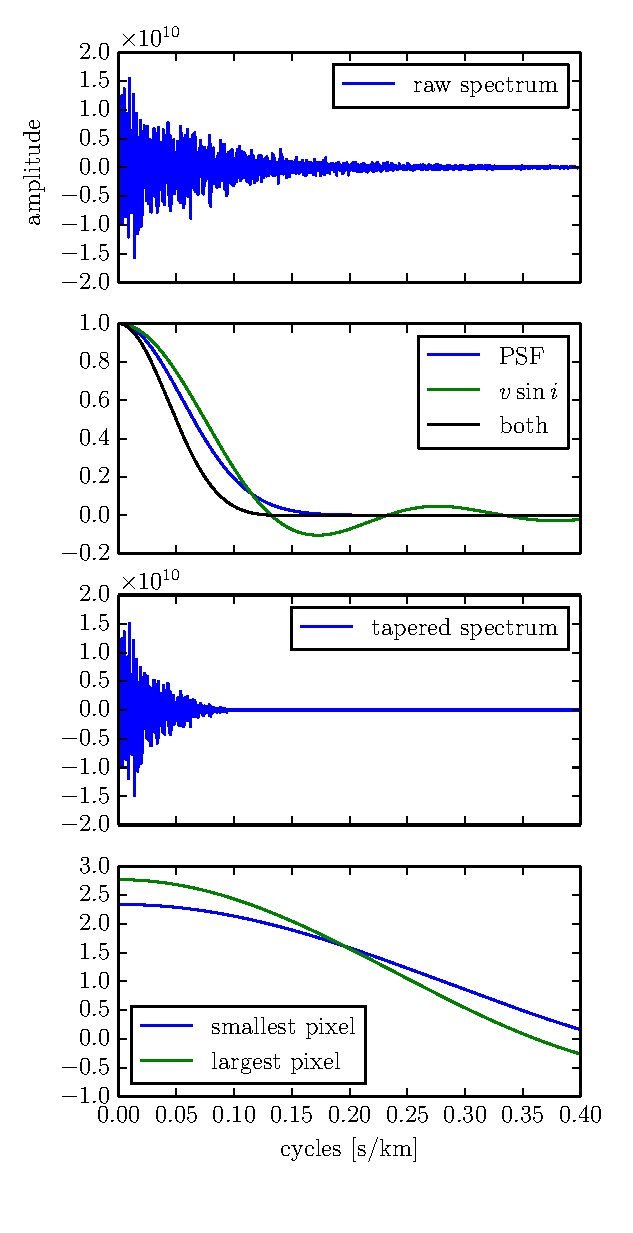
\includegraphics[width=0.5\textwidth]{pixel_response}
\caption{Pixel response}
\label{fig:pixel_response}
\end{center}
\end{figure}

In the future, we may consider doing away with the FFT routine entirely in favour of a sliding convolution approach, where the resolution of the kernel can change with wavelength, the way the actual PSF changes on the spectrograph.

\subsection{Pixel-convolved PSF}

The previous approach is not very rigorous about the distinction between intensity and flux. In your blog and papers you've mentioned the ``pixel-convolved'' PSF at the focal plane, or the ``pixel-beam.'' I was wondering if you could point me to a reference explaining the concept that makes prodigious use of equations? I've worked out the following\ldots could you point out anywhere I have gone wrong?

The intensity field $I(\vec{x}, \vec{n})$ is a function of three dimensional space and direction, denoted by a position vector $\vec{x}$ and direction vector $\vec{n}$.  In a spectrograph, this intensity field is modified by the system response of the dispersive mechanism, called the line spread function or point spread function (PSF). Assuming monochromatic light, the intensity field behind the spectrograph can be written as
\begin{equation}
  I^\prime_\nu(\vec{x}, \vec{n}) = PSF_\nu(\vec{x}, \vec{n}) \otimes I_\nu(\vec{x}, \vec{n})
\end{equation}

What we care most about is the intensity field at the focal plane, 
\begin{equation}
  I_{\nu, {\rm FP}}(x, y, \vec{n}) = I^\prime_\nu(x, y, z=0, \vec{n})
\end{equation}
where $x$ and $y$ denote position on the 2D focal plane.

If we have a infinitesimal pixel with size $dA$, then in time $dt$ a source at an angle of $\theta$ and with angular size $d\Omega$ will deliver the following energy to the pixel
\begin{equation}
  dE = I_\nu dt (dA \cos \theta) d\Omega d\nu
\end{equation}

My impression is that the ``pixel-beam'' becomes important when we consider that each pixel is not infinitesimal in size nor does it have a uniform response throughout the pixel nor to all directions of incoming light. If we define a directional pixel efficiency as $\eta_\nu(x, y, \vec{n})$, then the energy received by a pixel with finite area is
\begin{equation}
  E = \int \iint \int \int I_{\nu, {\rm FP}} (x, y, \vec{n})\, dt\, (dx\,dy \cos \theta) \eta_\nu(x, y, \vec{n}) \cdot \vec{n} \, d\vec{n}\, d\nu
\end{equation}

where the spatial integral over $dx, dy$ spans the size of the pixel. By ``pixel-beam,'' do you mean something similar to $\eta_\nu$? I am interested in learning more about how this is done, but have been unable to find a detailed mathematical example. Of course, for spectra, there is the additional problem of extraction, or converting the 2D spectrum into a 1D spectrum.


\section{Correlated noise}
\begin{itemize}
  \item \hcom{systematic errors don't necessarily invalidate chi-squared if they can be treated as a noise with a non-trivial covariance matrix; they just make chi-squared not an independent sum of residuals weighted by inverse variances but because a dot-product through a non-trivial inverse covariance tensor.}
  \item \hcom{"more drastic than adding in noise" -- what about "adding in highly covariant and correlated noise"? That takes no more equipment (everything is still Gaussian), but can handle far worse situations.}
  \item \hcom{Where you mention $\chi^2_Q$, you are treating the pixels as independent. But they aren't if there is model mismatch. That is, there are correlations among the residuals.}
\end{itemize}

Thank you for pointing this out. Your suggestions spurred a flurry of math on my part and I arrived at an interesting implementation of the correlated noise idea. When Dan Foreman-Mackey visited the CfA, I showed him my ideas and he gave me some great suggestions about to implement them in code.  

My first approach was to deal with the systematically bad regions of the spectrum, where there is a large, correlated residual due to a line strength mis-match. By approximating the residual as a Gaussian, I derived a covariance kernel which might parameterize the noise in this region.

If the mean function is
\begin{equation}
m(x) = E[f(x)]
\end{equation}
and the covariance function is
\begin{equation}
k(x, x^\prime) = E[(f(x) - m(x))(f(x^\prime) - m(x^\prime))]
\end{equation}
then we can compute the non-stationary covariance function describing a Gaussian as
\begin{equation}
k(x, x^\prime | a, \mu, \sigma) = \frac{a^2}{2 \pi \sigma} \exp \left ( - \frac{[(x - \mu)^2 + (x^\prime - \mu)^2]}{2 \sigma^2}\right )
\end{equation}


\begin{figure}[!htb]
\begin{center}
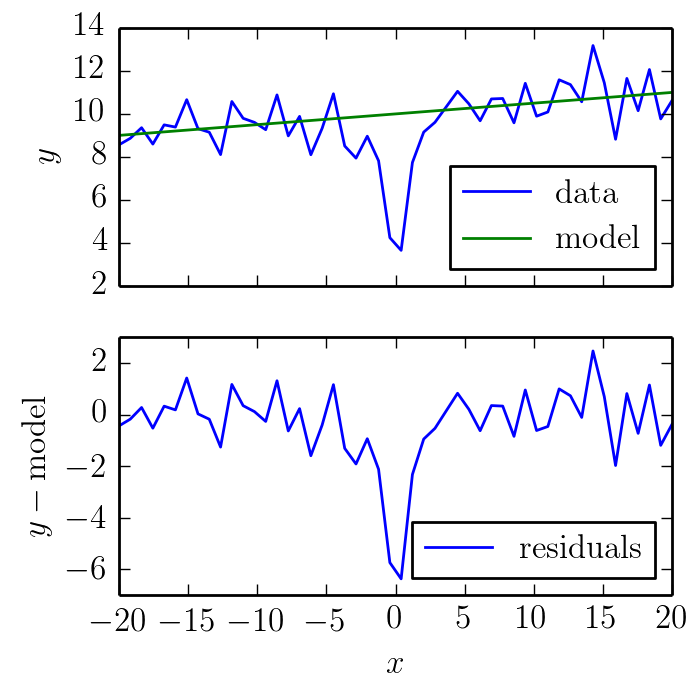
\includegraphics{fake_line}
\caption{A fake Gaussian residual}
\label{fig:fake_line}
\end{center}
\end{figure}

\begin{figure}[!htb]
\begin{center}
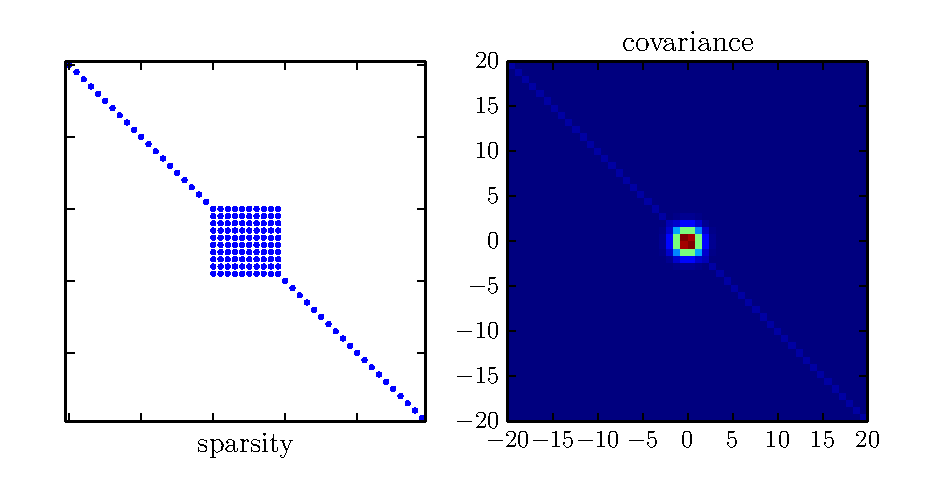
\includegraphics{matrix_region}
\caption{Left: sparsity. Right: covariance matrix with a Gaussian kernel as described above.}
\label{fig:matrix_region}
\end{center}
\end{figure}

Some text.

\begin{figure}[!htb]
\begin{center}
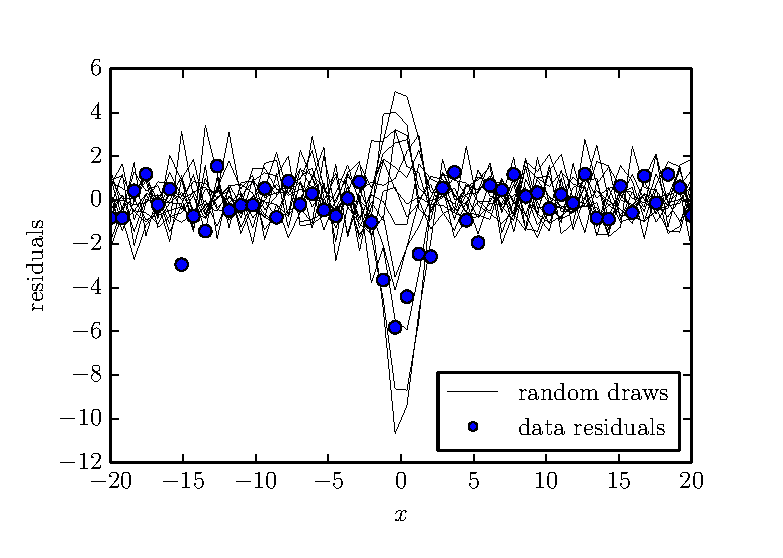
\includegraphics{random_draw}
\caption{15 random draws from the covariance matrix, overplotted with the residuals.}
\label{fig:random_draw}
\end{center}
\end{figure}

TODO: include simple figures showing that this covariance matrix can generate noise shaped like spectral lines. 

DFM recommended that we also implement a stationary covariance kernel to account for the general covariance structure of the data. For this, we use a Matern kernel \begin{equation}
  k_{\nu = 3/2}(r, a, l) = a \left(1 + \frac{\sqrt{3} r}{l} \right ) \exp \left (- \frac{\sqrt{3} r}{l} \right ) 
\end{equation}
and add compact support by tapering with a Haan window
\begin{equation}
  w(r) = 0.5 + 0.5 \cos \left( \frac{\pi r}{r_0} \right)
\end{equation}

When you look at a well-matched continuum region of the spectrum, the residuals are still correlated on a length scale.

For now we use wavelength, since this is easy to parameterize, and each wavelength corresponds to a pixel. This will be changed to velocity space soon.

\hcom{good on the stuff about there being important information where the models and data disagree.}

Point out that different covariance functions could be useful for different spectral problems, such as M dwarf continuum (show reference, or lifted plot).

By creating a new kernel with a finite bandwith, we can now 
We use a more general covariance function, which is the squared exponential with a Gaussian taper

\begin{equation}
k(x, x^\prime | h, a, \mu, \sigma) = \exp \left ( \frac{-( x - x^\prime)^2 }{2 h^2} \right ) \frac{a^2}{2 \pi \sigma} \exp \left ( - \frac{[(x - \mu)^2 + (x^\prime - \mu)^2]}{2 \sigma^2}\right )
\end{equation}
here $h$ is a "bandwidth" that controls the power of the oscillations. If $h$ is small, then there will be high-frequency structure. If $h$ is large, then only low-frequency structure will remain.

\begin{figure}[!htb]
\begin{center}
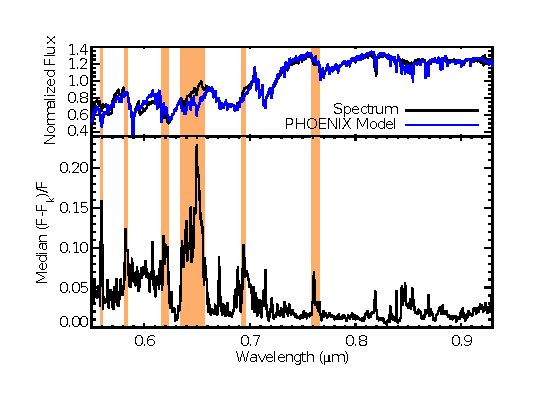
\includegraphics{mann}
\caption{From \citet{mga13}}
\label{fig:mann}
\end{center}
\end{figure}


\hcom{in your four classes of line behavior, there is none which is dominated by continuum issues? Or is there? That is, continuum fitting can cause problems, no?}
I would think that yes, there should be areas where continuum fitting can be a problem. However, in the stars I'm looking at (over the narrow echelle range), the Chebyshev formalism essentially assumes that any continuum mis-match is actually a flux-calibration (instrumental) issue, and accounts for it. This means that if we were fitting hotter stars with few lines, any information contained in the continuum shape would be lost. However, this approach does prevent against introducing bad features \emph{into} the continuum.

Depending on the size of the continuum problem, yes, this may also be a problem. I didn't include it in the error classification because I didn't think it was as dire a problem as the others, but when it comes to M spectra, this may actually be a problem.

\hcom{trigger went off with "making these regions useless for determining...". Useless?}
I shouldn't have been so hasty!

\hcom{Section 5: You might even be able to learn changes to the models. This is the holy grail.}

If we were to run against a large library of many stars (say, the \emph{Kepler} follow-up sample, or some SLOAN sample), we could use the learnt covariance of the spectrum to identify the bad regions and then determine how the models would need to be changed in order to fit all of the observed stars the best. I think this is similar to how the Johnson-Cousins photometric filter transmission profiles are reverse engineered (see Bessel and Murphy 2012 \S 3).


\section{Chebyshev}
\hcom{Can you really marginalize analytically over the Chebyshev polynomials? And doesn't that make a huge, correlated uncertainty tensor? And what priors do you use?}
I'm uncertain what you mean about the huge, correlated uncertainty tensor. Which parameters are in this tensor? 

Only four Chebyshevs per order.

\hcom{In re +/- 0.01 dex: You have tons of pixels so of course you get amazing constraints! It would be surprising if you didn't. But do you get such amazing constraints if you marginalize analytically over thousands of Chebyshevs?}
Show plot of run output, things still work fine, and in fact you get the same answer sampled vs. marginalized?

\hcom{When you do the drop and interpolate over testing, can you build an empirical interpolation error model and then use it?}
I am planning on building a model, but it has been lower priority at the moment. 






\bibliography{disks,bayesian,master}
\bibliographystyle{hapj}
\end{document}
